% \begin{preamble}
\documentclass[11pt]{article}
\usepackage[margin=1in]{geometry}
\usepackage[utf8]{inputenc}
\renewcommand{\rmdefault}{phv} % Arial Font
\renewcommand{\sfdefault}{phv} % Arial Font
\usepackage{color}
\usepackage{tcolorbox}
\usepackage{graphicx}
\usepackage{ragged2e}
\graphicspath{ {./figures/}} % Location of the graphics files
\usepackage[labelfont=bf]{caption}
\usepackage{multicol}
\usepackage{nopageno} % remove page numbers
\pagestyle{empty} % remove page numbers
\usepackage{gb4e}
\noautomath
% \end{preamble}

\newcommand{\glr}{\textcolor{teal}}
\definecolor{Purple}{RGB}{255,10,140}
\newcommand{\jd}[1]{\textcolor{Purple}{[jd: #1]}}


\begin{document}
% Title
\centerline{\textbf{A corpus-based study of (non-)exhaustivity in \emph{wh}-questions}}
% \centerline{Budgeting one line for names later} %names
% Endtitle 
A key issue in \emph{wh}-question interpretation regards the distribution of exhaustive (Mention-All, MA) vs. non-exhaustive (Mention-Some, MS) question readings (see (\ref{party}) and (\ref{coffee})): 
\begin{exe}
\hspace*{-\parindent}
    \begin{minipage}{0.45\linewidth}
        \ex Who came to the party?\label{party} 
            \vspace{-.1cm}
            \begin{xlist}
            \ex Who is every person that...? \hfill MA
            \vspace{-.1cm}
            \ex Who is a person that...? \hfill \#MS
            \vspace{-.1cm}
            \end{xlist}
    \end{minipage}
% \end{exe}
\hfill
% \begin{exe}
    \begin{minipage}{0.45\linewidth}
        \ex Where can I find coffee?\label{coffee}
            \vspace{-.1cm}
            \begin{xlist}
            \ex What is every place that...? \hfill MA
            \vspace{-.1cm}
            \ex What is a place that...? \hfill MS
            \vspace{-.1cm}
            \end{xlist}
    \end{minipage}
\end{exe}
\vspace{-.1cm}
Theories of question interpretation have typically assumed that a MA reading is always appropriate [1,2]. Linguistic factors that have been argued to generate variation in readings include the specific \emph{wh}-word---e.g., \emph{who}-questions are biased for MA, while \emph{where}/\emph{how}-questions are biased for MS [3-4]---and existential (priority) modality---e.g., \emph{can} purportedly licenses MS, as in (2) [5-9]. Recent work [10] tested these judgements in lab-controlled experiments with artificial stimuli and found evidence for some biases, but these biases can be overridden by features of the context like speaker/discourse goals [cf. 3-4,11]. However, there is to date no systematic investigation of \emph{naturally occurring questions} that tests the intuitions reported in the literature.  We ask: (Q1) How much does question interpretation vary in natural discourse contexts? Is there indeed a bias for MA? (Q2) Is the distribution of interpretations modulated by linguistic form? %We addressed these questions in a two-part study.

\textbf{Methods}.  \textbf{Step 1: Naturalistic Stimuli from a Corpus Database.}
Using TGrep2 and the Tgrep2 Database Tools [12-14], we extracted all occurrences of \emph{wh}-questions (10,009) from the Switchboard corpus [15] and coded the questions for syntactic structure (e.g., embedded, root), \emph{wh}-word, and presence of modality. To curate stimuli for step 2, we constrained the database to the most frequently discussed cases: root \emph{who}-, \emph{where}-, and \emph{how}-questions. We also removed degree (\emph{How much sugar do you need?}) and identity (\emph{Who is that?}) questions because MS and MA meanings converged, with 335 questions remaining. The distribution of \emph{wh}-word and modality in this database is reported in Table \ref{dist}.  \textbf{Step 2: Paraphrase Rating Task.} The remaining cases were divided into 11 lists with occurrence of critical factors roughly proportional to the overall database. Participants (n=385) on Prolific were presented with each question and the 10 preceding lines of dialogue, and asked to rate the likely intended meanings (paraphrases), using a slider task (Fig.~\ref{fig:stim}). Question paraphrases were selected to reflect MS/MA readings: \emph{a} indicates MS, \emph{every} MA, while in \emph{the}-paraphrase the two readings collapse. There was a fourth option (\emph{something else}) in case no other was appropriate. Performance on 6 catch trials functioned as exclusion criterion (n=19).

\textbf{Results.} Questions with highest ratings for \emph{something else} (17\%) were excluded because they were rhetorical (see Tab.~\ref{tab:exs}). \emph{The}-paraphrases, where MS=MA, had the highest mean rating (.59), suggesting that only one reading was possible for most cases. Data were analysed using linear mixed effects regression. To investigate the posited MA bias, we compared \emph{every} vs.~\emph{a} ratings, as these represent MA and MS (Fig.~\ref{fig:overall}): contrary to the literature, there was no bias for \emph{every} (Q1). However, significant two-way interactions between paraphrase and linguistic form factors 
partially support reports from the literature (Q2): first, the presence of a modal resulted in higher ratings of \emph{a} (p$<$.0001, Fig.~\ref{fig:modpres}) [5-9,10] but not \emph{every}. %, and marginally decreased ratings for \emph{the} (p=.07).
Second, ratings for \emph{how}-questions resulted in higher \emph{a} than \emph{every} ratings (p$<$.04), confirming [3-4, 10], but not for \emph{where} or \emph{who}-questions. %and reciprocally lower ratings for \emph{the} in both \emph{who} (p$<$.001) and \emph{how} (p$<$.0001) compared to \emph{where}. 

% \color{red}With respect to linguistic form (Q2): \emph{a} was rated higher than \emph{every} for modal questions (p$<$0.0001), in line with , but also with non-modal questions (p$<$0.0001) . INTERACTION\color{black} In line with [3-4], \emph{every} was rated lower than \emph{a} for \emph{how} (p$<$0.001)(Fig. \ref{fig:wh}), but--counter to [3-4]--not higher for \emph{who} (p=0.97).

% ModalPresence leads to greater MS
% How compared to where leads to MS

% Interactions para x modal:
% a: increase from red bar on right to red bar on left
% every: none
% the: marginal negative 

% greater prob of  MS if modal present


% interactions para x wh:
% for MS: wh doesn't change every (no effect relative to reference level)
% how: higher on a than on every; ms more available when wh is how
% who/where :no effect
% for the: going from where to how/who has negative effect

% We thus find that there's a greater probability of MS for modal questions and for \emph{how} questions.

\textbf{Conclusion.} In contrast to theoretical predictions, we find no bias for MA question readings in naturalistic dialogue (Q1). With respect to (Q2), we find support for some, but not all, observations about the effect of linguistic form on question interpretation reported in the literature. We suggest that MS/MA readings result from reasoning about the speaker's goal in the context, consistent with a constraint-based  account [16] on which hearers integrate multiple sources of information to determine meaning. These results also have methodological implications: data hand-selected during theory-building may be biased and not reflect a realistic distribution of meanings [17].


\newpage


\noindent
\begin{minipage}{0.6\linewidth}
\begin{tabular}{@{}|c|c|c|}
    \hline
    \textbf{Paraphrase} & \textbf{Example} & \textbf{Mean Rating}\\
    \hline
    \hline
    every & \emph{Where have you skied?} & .66\\
    (MA) & \emph{Where's it all going?} & .59 \\
    \hline
    a & \emph{Where do you like to eat?} & .57\\
    (MS) & \emph{How would you achieve that?} & .51\\
    \hline
    the & \emph{Where you going to school?} & .99\\
    (MS=MA) & \emph{Where do you work?} & .99\\
    \hline
    something & \emph{Who knows?} & .61\\
    else & \emph{How can you watch that?} & .53\\
    \hline
\end{tabular}
\vspace{-.3cm}
\captionof{table}{For each paraphrase, examples of questions that resulted in high ratings on that paraphrase.}
\label{tab:exs}
\end{minipage}
\hfill
\begin{minipage}{0.34\linewidth}
    \centering
    \begin{tabular}{@{}|c|c|c|}
    \hline
    \textbf{Wh} & \textbf{Modal?} & \textbf{\% of Total}\\
    \hline
    \hline
    \emph{who}  & Yes & 2.4\% \\
    {} & No & 13.7\%\\
    \hline
    \emph{where} & Yes & 1.2\%\\
    {} & No & 27.8\%\\
    \hline
    \emph{how} & Yes & 8.4\%\\
    {} & No & 46.6\%\\
    \hline
    \end{tabular}
    \captionof{table}{Joint distribution of \emph{wh}-words and modals in database of 335 root questions.}
    \label{dist}
\end{minipage}
\vspace{-.1cm}
\begin{tcolorbox}[colback=white]
% \hspace*{-\parindent}
\vspace{-.2cm}
\noindent 
\begin{minipage}{0.73\linewidth}
    \vspace{-.2cm}
    \hspace*{-.4cm}
    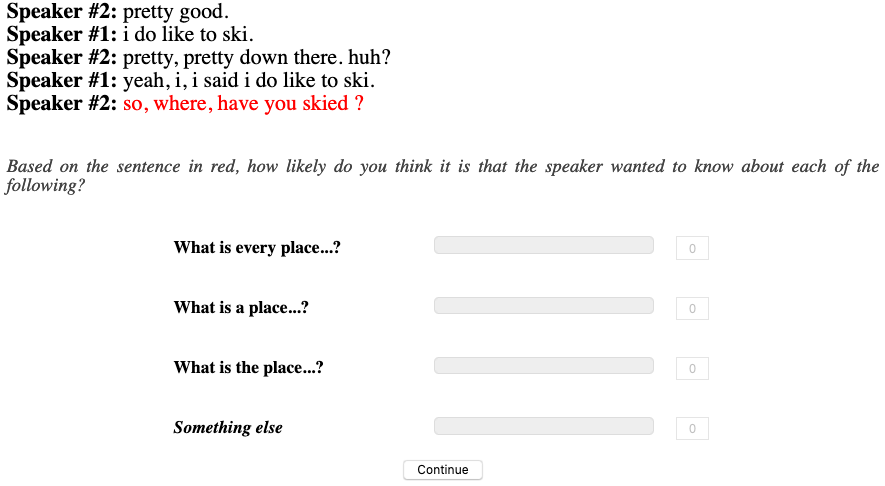
\includegraphics[scale=0.39]{figures/stim.png}
    \vspace{-.5cm}
\end{minipage}
\hfill
\hspace*{.45cm}
\begin{minipage}{0.23\linewidth}
    % \hspace*{.4cm}
% \vspace{-.2cm}
    \captionof{figure}{Paraphrase Rating Task: Participants evaluate intended question meanings by moving the slider next to paraphrases, assigning a numerical value between 0-1. Combined ratings must sum to 1 to generate a proper probability distribution.}
    \label{fig:stim}
    \vspace{-.3cm}
\end{minipage}
\vspace{-.3cm}
\end{tcolorbox}

\noindent
\begin{minipage}{0.32\linewidth}
\begin{tcolorbox}[colback=white]
    \hspace*{-.2cm}
    % \centering
    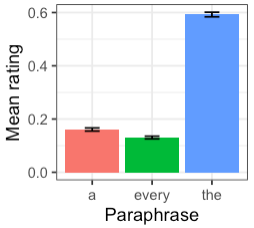
\includegraphics[scale=0.5]{figures/overall.png}
    \vspace{-.4cm}
    \centering
    \captionof{figure}{Surprisingly, \emph{every} paraphrases were not preferred over \emph{a} paraphrases.}
    \label{fig:overall}
\end{tcolorbox}
\end{minipage}
\hfill
\begin{minipage}{0.32\linewidth}
    \begin{tcolorbox}[colback=white]
    \vspace{-.2cm}
    \centering
    
\includegraphics[scale=0.6]{figures/legend.png}
    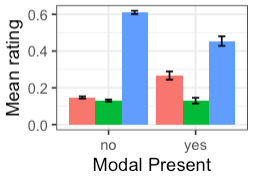
\includegraphics[scale=0.5]{figures/modpres.png}
    \vspace{-.6cm}
    \captionof{figure}{For modal questions, \emph{a} received higher ratings than \emph{every} (in line with [5-9]), but suprisingly not lower in non-modal questions (in contrast to [5-9]).}
    \label{fig:modpres}
    \vspace{-.2cm}
    \end{tcolorbox}
\end{minipage}
\hfill
\begin{minipage}{0.32\linewidth}
    \begin{tcolorbox}[colback=white]
    \vspace{-.2cm}
    \centering
    
\includegraphics[scale=0.6]{figures/legend.png}
    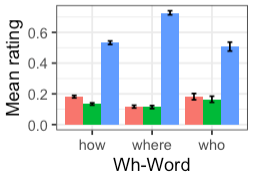
\includegraphics[scale=0.5]{figures/wh.png}
    \vspace{-.6cm}
    \captionof{figure}{\emph{A}-paraphrases received higher ratings than \emph{every} for \emph{how} (in line with [3-4]), but surprisingly not lower for \emph{who} (in contrast to [3-4]).}
    \label{fig:wh}
    \vspace{-.2cm}
    \end{tcolorbox}
\end{minipage}



\noindent \textbf{References}.
[1] Karttunen (1977),
[2] Groenendijk \& Stokhof (1984),
[3] Ginzburg (1995), 
[4] Asher \& Lascarides (1998), 
[5] George (2011), 
[6] Nicolae (2013), 
[7] Fox (2014), 
[8] Dayal (2016), 
[9] Xiang (2016), 
[10] Moyer \& Syrett (2019),
[11] van Rooij (2003),
[12] Rohde (2005), 
[13] Jaeger (2006), 
[14] Degen \& Jaeger (2011), 
[15] Godfrey et al. (1992), 
[16] Degen \& Tanenhaus (2019),
[17] Degen (2015)
\end{document}


% for writing up still run the modal on just "a" data